% This is a Basic Assignment Paper but with like Code and stuff allowed in it, there is also url, hyperlinks from contents included. 

\documentclass[11pt]{article}

% Preamble

\usepackage[margin=1in]{geometry}
\usepackage{amsfonts, amsmath, amssymb}
\usepackage{fancyhdr, float, graphicx}
\usepackage[utf8]{inputenc} % Required for inputting international characters
\usepackage[T1]{fontenc} % Output font encoding for international characters
\usepackage{fouriernc} % Use the New Century Schoolbook font
\usepackage[nottoc, notlot, notlof]{tocbibind}
\usepackage{listings}
\usepackage{xcolor}
\usepackage{blindtext}
\usepackage{hyperref}
\hypersetup{
    colorlinks=true,
    linkcolor=black,
    filecolor=magenta,      
    urlcolor=cyan,
    pdfpagemode=FullScreen,
    }

\definecolor{codegreen}{rgb}{0,0.6,0}
\definecolor{codegray}{rgb}{0.5,0.5,0.5}
\definecolor{codepurple}{rgb}{0.58,0,0.82}
\definecolor{backcolour}{rgb}{0.95,0.95,0.92}

\lstdefinestyle{mystyle}{
    backgroundcolor=\color{backcolour},   
    commentstyle=\color{codegreen},
    keywordstyle=\color{magenta},
    numberstyle=\tiny\color{codegray},
    stringstyle=\color{codepurple},
    basicstyle=\ttfamily\footnotesize,
    breakatwhitespace=false,         
    breaklines=true,                 
    captionpos=b,                    
    keepspaces=true,                 
    numbers=left,                    
    numbersep=5pt,                  
    showspaces=false,                
    showstringspaces=false,
    showtabs=false,                  
    tabsize=2
}

\lstset{style=mystyle}

% Header and Footer
\pagestyle{fancy}
\fancyhead{}
\fancyfoot{}
\fancyhead[L]{\textit{\Large{Database Management Systems Assignment 4}}}
%\fancyhead[R]{\textit{something}}
\fancyfoot[C]{\thepage}
\renewcommand{\footrulewidth}{1pt}



% Other Doc Editing
% \parindent 0ex
%\renewcommand{\baselinestretch}{1.5}

\begin{document}

\begin{titlepage}
	\centering

	%---------------------------NAMES-------------------------------

	\huge\textsc{
		MIT World Peace University
	}\\

	\vspace{0.75\baselineskip} % space after Uni Name

	\LARGE{
		Database Management Systems\\
		Second Year B. Tech, Semester 4
	}

	\vfill % space after Sub Name

	%--------------------------TITLE-------------------------------

	\rule{\textwidth}{1.6pt}\vspace*{-\baselineskip}\vspace*{2pt}
	\rule{\textwidth}{0.6pt}
	\vspace{0.75\baselineskip} % Whitespace above the title



	\huge{\textsc{
			Group Functions, Join and Nested Queries.
		}} \\



	\vspace{0.5\baselineskip} % Whitespace below the title
	\rule{\textwidth}{0.6pt}\vspace*{-\baselineskip}\vspace*{2.8pt}
	\rule{\textwidth}{1.6pt}

	\vspace{1\baselineskip} % Whitespace after the title block

	%--------------------------SUBTITLE --------------------------	

	\LARGE\textsc{
		Assignment No. 4
	} % Subtitle or further description
	\vfill

	%--------------------------AUTHOR-------------------------------

	Prepared By
	\vspace{0.5\baselineskip} % Whitespace before the editors

	\Large{
		Krishnaraj Thadesar \\
		Cyber Security and Forensics\\
		Batch A1, PA 20
	}


	\vspace{0.5\baselineskip} % Whitespace below the editor list
	\today

\end{titlepage}


\tableofcontents
\thispagestyle{empty}
\clearpage

\setcounter{page}{1}

\section{Aim}
Write suitable select command to get requested data from tables

\section{Objectives}
\begin{enumerate}
	\item To study Subqueries, Group, Joins and Views
\end{enumerate}

\section{Problem Statement}
Create tables and solve given queries using , Group, Joins and Views

\section{Theory}

\subsection{Group Functions}
Group functions in SQL are functions that operate on groups of rows in a table, and return a single result for each group. They are often used in conjunction with the GROUP BY clause, which divides a table into groups based on one or more columns, and applies the group functions to each group.

The common group functions in SQL are:



\begin{enumerate}
	\item COUNT - Counts the number of rows in a group.
	\item SUM - Calculates the sum of a column in a group.
	\item AVG - Calculates the average value of a column in a group.
	\item MIN - Finds the minimum value of a column in a group.
	\item MAX - Finds the maximum value of a column in a group.
\end{enumerate}


\textbf{Syntax: }

\begin{lstlisting}[language=sql]
SELECT column_name, group_function(column_name)
FROM table_name
WHERE condition
GROUP BY column_name;
\end{lstlisting}

\textbf{Example: }

Consider the following table "employees":

\begin{table}[H]
	\begin{tabular}{llll}
		\textbf{id} & \textbf{name} & \textbf{department} & \textbf{salary} \\
		1           & Alice         & HR                  & 5000            \\
		2           & Bob           & IT                  & 6000            \\
		3           & Charlie       & HR                  & 4500            \\
		4           & David         & IT                  & 7000            \\
		5           & Emma          & Sales               & 5500
	\end{tabular}
\end{table}

\textit{To count the number of employees in each department, you can use the following query:}

\begin{lstlisting}[language=sql]
SELECT department, COUNT(*)
FROM employees
GROUP BY department;
\end{lstlisting}


\begin{table}[H]
	\begin{tabular}{ll}
		\textbf{department} & \textbf{COUNT(*)} \\
		HR                  & 2                 \\
		IT                  & 2                 \\
		Sales               & 1
	\end{tabular}
\end{table}


\textit{To find the average salary of employees in each department, you can use the following query:}

\begin{lstlisting}[language=sql]
SELECT department, AVG(salary)
FROM employees
GROUP BY department;
\end{lstlisting}


\begin{table}[H]
	\begin{tabular}{ll}
		\textbf{department} & \textbf{AVG(salary)} \\
		HR                  & 4750                 \\
		IT                  & 6500                 \\
		Sales               & 5500
	\end{tabular}
\end{table}


\textit{To find the maximum salary in the entire table, you can use the following query:}

\begin{lstlisting}[language=sql]
SELECT MAX(salary)
FROM employees;
\end{lstlisting}

\begin{table}[H]
	\begin{tabular}{l}
		\textbf{MAX(salary)} \\
		7000
	\end{tabular}
\end{table}

\subsection{SQL Join Types}

In SQL, join is used to combine two or more tables based on a common column between them. There are several types of joins in SQL, each with its own syntax and usage.

\textit{Consider the Following Tables}

\begin{lstlisting}[language=sql]
	MariaDB [dbms_lab]> select * from booking;
	+---------+---------+------------+------------+--------+
	| HotelNo | GuestNo | DateFrom   | DateTo     | RoomNo |
	+---------+---------+------------+------------+--------+
	|       7 |      10 | 2096-04-21 | 2099-12-21 |     10 |
	|       8 |       5 | 2077-09-29 | 2109-09-10 |     11 |
	|      11 |       4 | 2123-01-05 | 2063-08-30 |      2 |
	|      10 |       5 | 2027-02-05 | 2119-12-21 |      7 |
	|       9 |       5 | 2081-07-11 | 2031-06-20 |     13 |
	|       5 |       5 | 2059-11-19 | 2113-05-22 |     11 |
	+---------+---------+------------+------------+--------+
	6 rows in set (0.001 sec)
	
	MariaDB [dbms_lab]> select * from Hotel;
	+---------+------------------+-----------------------+
	| HotelNo | Name             | City                  |
	+---------+------------------+-----------------------+
	|       1 | Hotel love       | Guernsey              |
	|       2 | Hotel imagine    | Jordan                |
	|       3 | Hotel rice       | Equatorial Guinea     |
	|       4 | Hotel perhaps    | Bolivia               |
	|       5 | Hotel show       | Reunion               |
	|       6 | Hotel native     | Brunei                |
	|       7 | Hotel pool       | Panama                |
	|       8 | Hotel spin       | Guyana                |
	|       9 | Hotel toward     | St. Barthelemy        |
	|      10 | Hotel expression | St. Pierre & Miquelon |
	|      11 | Hotel cheese     | Guinea-Bissau         |
	|      12 | Hotel motion     | Latvia                |
	|      13 | Hotel lay        | Fiji                  |
	|      14 | Hotel stiff      | Brazil                |
	|      15 | Hotel suddenly   | Lithuania             |
	|      16 | Hotel stretch    | Montenegro            |
	|      17 | Hotel current    | Isle of Man           |
	|      18 | Hotel forest     | Haiti                 |
	+---------+------------------+-----------------------+
	18 rows in set (0.001 sec)
\end{lstlisting}

\subsection{Inner Join or Simple Join}

\subsubsection*{Defintion}

The inner join is used to select all matching rows or columns in both tables or as long as the defined condition is valid in SQL.

\subsubsection*{Figure}

\begin{figure}[H]
	\centering
	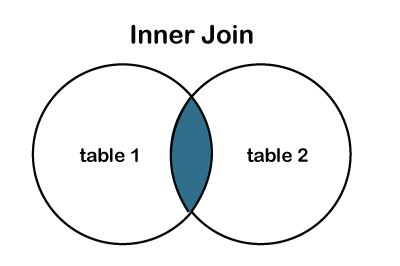
\includegraphics[width=.45\textwidth]{inner join.png}
	\caption{ Inner Join}
\end{figure}

\subsubsection*{Syntax}

\begin{lstlisting}[language=sql]
Select column_1, column_2, column_3 FROM table_1 INNER JOIN table_2 ON table_1.column = table_2.column; 
\end{lstlisting}

\subsubsection*{Example}

\begin{lstlisting}[language=sql]
MariaDB [dbms_lab]> select booking.HotelNo, Hotel.name from booking inner join Hotel on booking.HotelNo = Hotel.HotelNo;
+---------+------------------+
| HotelNo | name             |
+---------+------------------+
|       5 | Hotel show       |
|       7 | Hotel pool       |
|       8 | Hotel spin       |
|       9 | Hotel toward     |
|      10 | Hotel expression |
|      11 | Hotel cheese     |
+---------+------------------+
6 rows in set (0.001 sec)
\end{lstlisting}

\subsection{Left Join}

\subsubsection*{Defintion}

The LEFT JOIN is used to retrieve all records from the left table (table1) and the matched rows or columns from the right table (table2). If both tables do not contain any matched rows or columns, it returns the NULL.

\subsubsection*{Figure}

\begin{figure}[H]
	\centering
	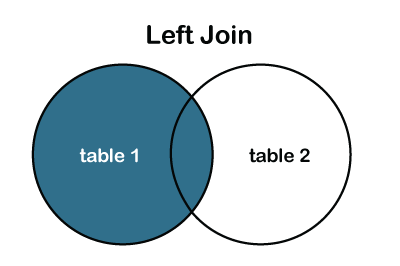
\includegraphics[width=.45\textwidth]{left join.png}
	\caption{ Left Join}
\end{figure}

\subsubsection*{Syntax}

\begin{lstlisting}[language=sql]
Select column_1, column_2, column(s) FROM table_1 LEFT JOIN table_2 ON table_1.column_name = table_2.column_name;  
\end{lstlisting}

\subsubsection*{Example}

\begin{lstlisting}[language=sql]
MariaDB [dbms_lab]> select * from booking left join Hotel on booking.HotelNo = Hotel.HotelNo;
+--------+---------+------------------+-----------------------+
| RoomNo | HotelNo | Name             | City                  |
+--------+---------+------------------+-----------------------+
|     10 |       7 | Hotel pool       | Panama                |
|     11 |       8 | Hotel spin       | Guyana                |
|      2 |      11 | Hotel cheese     | Guinea-Bissau         |
|      7 |      10 | Hotel expression | St. Pierre & Miquelon |
|     13 |       9 | Hotel toward     | St. Barthelemy        |
|     11 |       5 | Hotel show       | Reunion               |
+--------+---------+------------------+-----------------------+
6 rows in set (0.001 sec)
\end{lstlisting}

\subsection{Right Join}

\subsubsection*{Defintion}

The RIGHT JOIN is used to retrieve all records from the right table (table2) and the matched rows or columns from the left table (table1). If both tables do not contain any matched rows or columns, it returns the NULL.

\subsubsection*{Figure}

\begin{figure}[H]
	\centering
	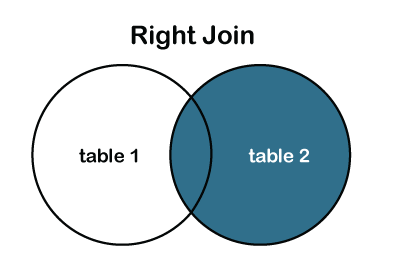
\includegraphics[width=.45\textwidth]{right join.png}
	\caption{ Right Join}
\end{figure}

\subsubsection*{Syntax}

\begin{lstlisting}[language=sql]
Select column_1, column_2, column_3 FROM table_1 RIGHT JOIN table_2 ON table_1.column = table_2.column; 
\end{lstlisting}

\subsubsection*{Example}

\begin{lstlisting}[language=sql]

MariaDB [dbms_lab]> select * from booking right join Hotel on booking.HotelNo = Hotel.HotelNo;
+--------+---------+------------------+-----------------------+
| RoomNo | HotelNo | Name             | City                  |
+--------+---------+------------------+-----------------------+
|     10 |       7 | Hotel pool       | Panama                |
|     11 |       8 | Hotel spin       | Guyana                |
|      2 |      11 | Hotel cheese     | Guinea-Bissau         |
|      7 |      10 | Hotel expression | St. Pierre & Miquelon |
|     13 |       9 | Hotel toward     | St. Barthelemy        |
|     11 |       5 | Hotel show       | Reunion               |
|   NULL |       1 | Hotel love       | Guernsey              |
|   NULL |       2 | Hotel imagine    | Jordan                |
|   NULL |       3 | Hotel rice       | Equatorial Guinea     |
|   NULL |       4 | Hotel perhaps    | Bolivia               |
|   NULL |       6 | Hotel native     | Brunei                |
|   NULL |      12 | Hotel motion     | Latvia                |
|   NULL |      13 | Hotel lay        | Fiji                  |
|   NULL |      14 | Hotel stiff      | Brazil                |
|   NULL |      15 | Hotel suddenly   | Lithuania             |
|   NULL |      16 | Hotel stretch    | Montenegro            |
|   NULL |      17 | Hotel current    | Isle of Man           |
|   NULL |      18 | Hotel forest     | Haiti                 |
+--------+---------+------------------+-----------------------+
18 rows in set (0.002 sec)
\end{lstlisting}

\subsection{Natural Join}

\subsubsection*{Defintion}

It is a type of inner type that joins two or more tables based on the same column name and has the same data type present on both tables.

\subsubsection*{Syntax}

\begin{lstlisting}[language=sql]
Select * from tablename1 Natural JOIN tablename_2;  
\end{lstlisting}

\subsubsection*{Example}

\begin{lstlisting}[language=sql]
MariaDB [dbms_lab]> select * from booking natural join Hotel
-> ;
+--------+------------------+-----------------------+
| RoomNo | Name             | City                  |
+--------+------------------+-----------------------+
|     10 | Hotel pool       | Panama                |
|     11 | Hotel spin       | Guyana                |
|      2 | Hotel cheese     | Guinea-Bissau         |
|      7 | Hotel expression | St. Pierre & Miquelon |
|     13 | Hotel toward     | St. Barthelemy        |
|     11 | Hotel show       | Reunion               |
+--------+------------------+-----------------------+
6 rows in set (0.001 sec)
\end{lstlisting}

\subsection{Full Outer Join}

\subsubsection*{Defintion}

It is a combination result set of both LEFT JOIN and RIGHT JOIN. The joined tables return all records from both the tables and if no matches are found in the table, it places NULL. It is also called a FULL OUTER JOIN.


\subsubsection*{Figure}

\begin{figure}[H]
	\centering
	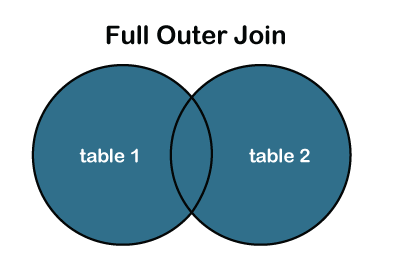
\includegraphics[width=.45\textwidth]{full outer join.png}
	\caption{ Right Join}
\end{figure}

\subsubsection*{Syntax}

\begin{lstlisting}[language=sql]
	Select column_1, column_2, column(s) FROM table_1 FULL JOIN table_2 ON table_1.column_name = table_2.column_name;  
\end{lstlisting}

\subsubsection*{Example}

\begin{lstlisting}[language=sql]

MariaDB [dbms_lab]> select * from booking left join Hotel on booking.HotelNo = Hotel.HotelNo
-> union
-> select * from booking right join Hotel on booking.HotelNo = Hotel.HotelNo;
+--------+---------+------------------+-----------------------+
| RoomNo | HotelNo | Name             | City                  |
+--------+---------+------------------+-----------------------+
|     10 |       7 | Hotel pool       | Panama                |
|     11 |       8 | Hotel spin       | Guyana                |
|      2 |      11 | Hotel cheese     | Guinea-Bissau         |
|      7 |      10 | Hotel expression | St. Pierre & Miquelon |
|     13 |       9 | Hotel toward     | St. Barthelemy        |
|     11 |       5 | Hotel show       | Reunion               |
|   NULL |       1 | Hotel love       | Guernsey              |
|   NULL |       2 | Hotel imagine    | Jordan                |
|   NULL |       3 | Hotel rice       | Equatorial Guinea     |
|   NULL |       4 | Hotel perhaps    | Bolivia               |
|   NULL |       6 | Hotel native     | Brunei                |
|   NULL |      12 | Hotel motion     | Latvia                |
|   NULL |      13 | Hotel lay        | Fiji                  |
|   NULL |      14 | Hotel stiff      | Brazil                |
|   NULL |      15 | Hotel suddenly   | Lithuania             |
|   NULL |      16 | Hotel stretch    | Montenegro            |
|   NULL |      17 | Hotel current    | Isle of Man           |
|   NULL |      18 | Hotel forest     | Haiti                 |
+--------+---------+------------------+-----------------------+
18 rows in set (0.008 sec)
\end{lstlisting}

\subsection{Cross Join}

\subsubsection*{Defintion}

It is also known as CARTESIAN JOIN, which returns the Cartesian product of two or more joined tables. The CROSS JOIN produces a table that merges each row from the first table with each second table row. It is not required to include any condition in CROSS JOIN.

\subsubsection*{Syntax}

\begin{lstlisting}[language=sql]
Select * from table_1 cross join table_2;  
\end{lstlisting}

\subsubsection*{Example}

\begin{lstlisting}[language=sql]

MariaDB [dbms_lab]>
MariaDB [dbms_lab]> select booking.HotelNo, booking.RoomNo, Hotel.name, Hotel.City from booking cross join Hotel;
+---------+--------+------------------+-----------------------+
| HotelNo | RoomNo | name             | City                  |
+---------+--------+------------------+-----------------------+
|       7 |     10 | Hotel love       | Guernsey              |
|       8 |     11 | Hotel love       | Guernsey              |
|      11 |      2 | Hotel love       | Guernsey              |
|      10 |      7 | Hotel love       | Guernsey              |
|       9 |     13 | Hotel love       | Guernsey              |
|       5 |     11 | Hotel love       | Guernsey              |
|       7 |     10 | Hotel imagine    | Jordan                |
|       8 |     11 | Hotel imagine    | Jordan                |
|      11 |      2 | Hotel imagine    | Jordan                |
|      10 |      7 | Hotel imagine    | Jordan                |
|       9 |     13 | Hotel imagine    | Jordan                |
|       5 |     11 | Hotel imagine    | Jordan                |
|       7 |     10 | Hotel rice       | Equatorial Guinea     |
|       8 |     11 | Hotel rice       | Equatorial Guinea     |
|      11 |      2 | Hotel rice       | Equatorial Guinea     |
|      10 |      7 | Hotel rice       | Equatorial Guinea     |
|       9 |     13 | Hotel rice       | Equatorial Guinea     |
|       5 |     11 | Hotel rice       | Equatorial Guinea     |
|       7 |     10 | Hotel perhaps    | Bolivia               |
|       8 |     11 | Hotel perhaps    | Bolivia               |
|      11 |      2 | Hotel perhaps    | Bolivia               |
|      10 |      7 | Hotel perhaps    | Bolivia               |
|       9 |     13 | Hotel perhaps    | Bolivia               |
|       5 |     11 | Hotel perhaps    | Bolivia               |
|       7 |     10 | Hotel show       | Reunion               |
|       8 |     11 | Hotel show       | Reunion               |
|      11 |      2 | Hotel show       | Reunion               |
|      10 |      7 | Hotel show       | Reunion               |
|       9 |     13 | Hotel show       | Reunion               |
|       5 |     11 | Hotel show       | Reunion               |
|       7 |     10 | Hotel native     | Brunei                |
|       8 |     11 | Hotel native     | Brunei                |
|      11 |      2 | Hotel native     | Brunei                |
|      10 |      7 | Hotel native     | Brunei                |
|       9 |     13 | Hotel native     | Brunei                |
|       5 |     11 | Hotel native     | Brunei                |
|       7 |     10 | Hotel pool       | Panama                |
|       8 |     11 | Hotel pool       | Panama                |
|      11 |      2 | Hotel pool       | Panama                |
|      10 |      7 | Hotel pool       | Panama                |
|       9 |     13 | Hotel pool       | Panama                |
|       5 |     11 | Hotel pool       | Panama                |
|       7 |     10 | Hotel spin       | Guyana                |
|       8 |     11 | Hotel spin       | Guyana                |
|      11 |      2 | Hotel spin       | Guyana                |
|      10 |      7 | Hotel spin       | Guyana                |
|       9 |     13 | Hotel spin       | Guyana                |
|       5 |     11 | Hotel spin       | Guyana                |
|       7 |     10 | Hotel toward     | St. Barthelemy        |
|       8 |     11 | Hotel toward     | St. Barthelemy        |
|      11 |      2 | Hotel toward     | St. Barthelemy        |
|      10 |      7 | Hotel toward     | St. Barthelemy        |
|       9 |     13 | Hotel toward     | St. Barthelemy        |
|       5 |     11 | Hotel toward     | St. Barthelemy        |
|       7 |     10 | Hotel expression | St. Pierre & Miquelon |
|       8 |     11 | Hotel expression | St. Pierre & Miquelon |
|      11 |      2 | Hotel expression | St. Pierre & Miquelon |
|      10 |      7 | Hotel expression | St. Pierre & Miquelon |
|       9 |     13 | Hotel expression | St. Pierre & Miquelon |
|       5 |     11 | Hotel expression | St. Pierre & Miquelon |
|       7 |     10 | Hotel cheese     | Guinea-Bissau         |
|       8 |     11 | Hotel cheese     | Guinea-Bissau         |
|      11 |      2 | Hotel cheese     | Guinea-Bissau         |
|      10 |      7 | Hotel cheese     | Guinea-Bissau         |
|       9 |     13 | Hotel cheese     | Guinea-Bissau         |
|       5 |     11 | Hotel cheese     | Guinea-Bissau         |
|       7 |     10 | Hotel motion     | Latvia                |
|       8 |     11 | Hotel motion     | Latvia                |
|      11 |      2 | Hotel motion     | Latvia                |
|      10 |      7 | Hotel motion     | Latvia                |
|       9 |     13 | Hotel motion     | Latvia                |
|       5 |     11 | Hotel motion     | Latvia                |
|       7 |     10 | Hotel lay        | Fiji                  |
|       8 |     11 | Hotel lay        | Fiji                  |
|      11 |      2 | Hotel lay        | Fiji                  |
|      10 |      7 | Hotel lay        | Fiji                  |
|       9 |     13 | Hotel lay        | Fiji                  |
|       5 |     11 | Hotel lay        | Fiji                  |
|       7 |     10 | Hotel stiff      | Brazil                |
|       8 |     11 | Hotel stiff      | Brazil                |
|      11 |      2 | Hotel stiff      | Brazil                |
|      10 |      7 | Hotel stiff      | Brazil                |
|       9 |     13 | Hotel stiff      | Brazil                |
|       5 |     11 | Hotel stiff      | Brazil                |
|       7 |     10 | Hotel suddenly   | Lithuania             |
|       8 |     11 | Hotel suddenly   | Lithuania             |
|      11 |      2 | Hotel suddenly   | Lithuania             |
|      10 |      7 | Hotel suddenly   | Lithuania             |
|       9 |     13 | Hotel suddenly   | Lithuania             |
|       5 |     11 | Hotel suddenly   | Lithuania             |
|       7 |     10 | Hotel stretch    | Montenegro            |
|       8 |     11 | Hotel stretch    | Montenegro            |
|      11 |      2 | Hotel stretch    | Montenegro            |
|      10 |      7 | Hotel stretch    | Montenegro            |
|       9 |     13 | Hotel stretch    | Montenegro            |
|       5 |     11 | Hotel stretch    | Montenegro            |
|       7 |     10 | Hotel current    | Isle of Man           |
|       8 |     11 | Hotel current    | Isle of Man           |
|      11 |      2 | Hotel current    | Isle of Man           |
|      10 |      7 | Hotel current    | Isle of Man           |
|       9 |     13 | Hotel current    | Isle of Man           |
|       5 |     11 | Hotel current    | Isle of Man           |
|       7 |     10 | Hotel forest     | Haiti                 |
|       8 |     11 | Hotel forest     | Haiti                 |
|      11 |      2 | Hotel forest     | Haiti                 |
|      10 |      7 | Hotel forest     | Haiti                 |
|       9 |     13 | Hotel forest     | Haiti                 |
|       5 |     11 | Hotel forest     | Haiti                 |
+---------+--------+------------------+-----------------------+
108 rows in set (0.000 sec)
\end{lstlisting}

\subsection{Self Join}

\subsubsection*{Defintion}

It is a SELF JOIN used to create a table by joining itself as there were two tables. It makes temporary naming of at least one table in an SQL statement.

\subsubsection*{Syntax}

\begin{lstlisting}[language=sql]
	Select column1, column2, column(s) FROM table_1 Tbl1, table_1 Tbl2 WHERE condition;  
\end{lstlisting}

\section{Platform}
\textbf{Operating System}: Arch Linux x86-64 \\
\textbf{IDEs or Text Editors Used}: Draw.io for Drawing the ER diagram.

% \section{Pseudo Code or Algorithm}

\section{Input}
Given Database from the Problem Statement for the Assignment for our batch. (A1 PA 20)

\section{Executed Queries}

\subsection{Questions SetA}

\lstinputlisting[language=SQL]{../../Programs/Assignment_4.md}

\subsection{Questions Set B}

\lstinputlisting[language=SQL]{../../Programs/Assignment_4_part_2.md}


\section{Conclusion}
Thus, we have learned to Select Group By, Joins and Subqueries commands thoroughly.
\clearpage

\section{FAQ}
\begin{enumerate}
	\item \textbf{When to use self join? How does it differ from other joins?}\\

	      A self join is used when you need to join a table with itself, typically to find relationships between rows in the same table. It differs from other joins in that you are joining a table with itself rather than joining two separate tables. A self join can be performed using an alias to distinguish between the two copies of the table being joined.


	      \begin{lstlisting}[language=sql]
SELECT t1.employee_name, t2.employee_name 
FROM employees t1 
JOIN employees t2 ON t1.manager_id = t2.employee_id;
\end{lstlisting}

	\item \textbf{Compare Cross Join with Natural Join. Share your comments.}\\

	      A cross join produces the Cartesian product of two tables, resulting in a combination of all rows from one table with all rows from another table. A natural join matches two tables based on their common column names. It automatically eliminates duplicate columns from the result set, and the result set only contains the columns with the same name from both tables.

	      \begin{lstlisting}[language=sql]
	SELECT *
	FROM table1
	CROSS JOIN table2;
\end{lstlisting}

	\item \textbf{What is the importance of SQL joins in database management? Explain its types.}\\

	      SQL joins are important in database management because they allow you to combine data from two or more tables into a single result set. This allows you to extract meaningful information from your data by revealing relationships between tables. There are four main types of SQL joins: inner join, left join, right join, and full outer join.


	\item \textbf{What are the different types of Joins in SQL?}\\

	      The different types of SQL joins are:

	      \begin{itemize}
		      \item Inner join: returns only the matching rows from both tables based on the specified join condition.

		      \item Left join: returns all the rows from the left table and the matching rows from the right table based on the specified join condition.

		      \item Right join: returns all the rows from the right table and the matching rows from the left table based on the specified join condition.

		      \item Full outer join: returns all the rows from both tables, matching rows where possible and filling in NULL values for non-matching rows.

	      \end{itemize}

	      \begin{lstlisting}[language=sql]
SELECT *
FROM table1
INNER JOIN table2
ON table1.column = table2.column;
	\end{lstlisting}

	      \begin{lstlisting}[language=sql]
SELECT *
FROM table1
LEFT JOIN table2
ON table1.column = table2.column;
\end{lstlisting}



	\item \textbf{State the difference between inner join and left join.}\\

	      The main difference between an inner join and a left join is that an inner join only returns matching rows from both tables based on the specified join condition, while a left join returns all the rows from the left table and the matching rows from the right table based on the specified join condition.

	      \begin{lstlisting}[language=sql]
SELECT *
FROM table1
LEFT JOIN table2
ON table1.column = table2.column;
\end{lstlisting}

	      \begin{lstlisting}[language=sql]
SELECT *
FROM table1
INNER JOIN table2
ON table1.column = table2.column;
\end{lstlisting}

	\item \textbf{State difference between left join and right join.}\\

	      The main difference between a left join and a right join is that a left join returns all the rows from the left table and the matching rows from the right table based on the specified join condition, while a right join returns all the rows from the right table and the matching rows from the left table based on the specified join condition.

	      \begin{lstlisting}[language=sql]
SELECT *
FROM table1
LEFT JOIN table2
ON table1.column = table2.column;
\end{lstlisting}

	      \begin{lstlisting}[language=sql]
SELECT *
FROM table1
RIGHT JOIN table2
ON table1.column = table2.column;
	\end{lstlisting}

\end{enumerate}


\end{document}